\section{Crossbar Array Architecture}
\label{sec:bg-crossbar}

Commercial OxRAM memories organize bitcells in a crossbar array, with
bitcells placed at the intersections of wordlines (WLs) and bitlines
(BLs)~\cite{wong2012metal}. WL and BL voltages are used to select and
bias individual cells for read and write operations. In practice, cells
are grouped into words that share a WL, and write operations are
performed at word granularity. The physical word size of the array is
the smallest unit that can be atomically programmed, and is determined
by the width of the write datapath in the memory controller. In
commercial standalone OxRAM products, the physical word size is not
disclosed in the device specification and must be inferred from timing
measurements, as demonstrated in Chapter~\ref{chap:brewrc}.

\begin{figure}[t!]
	\centering
	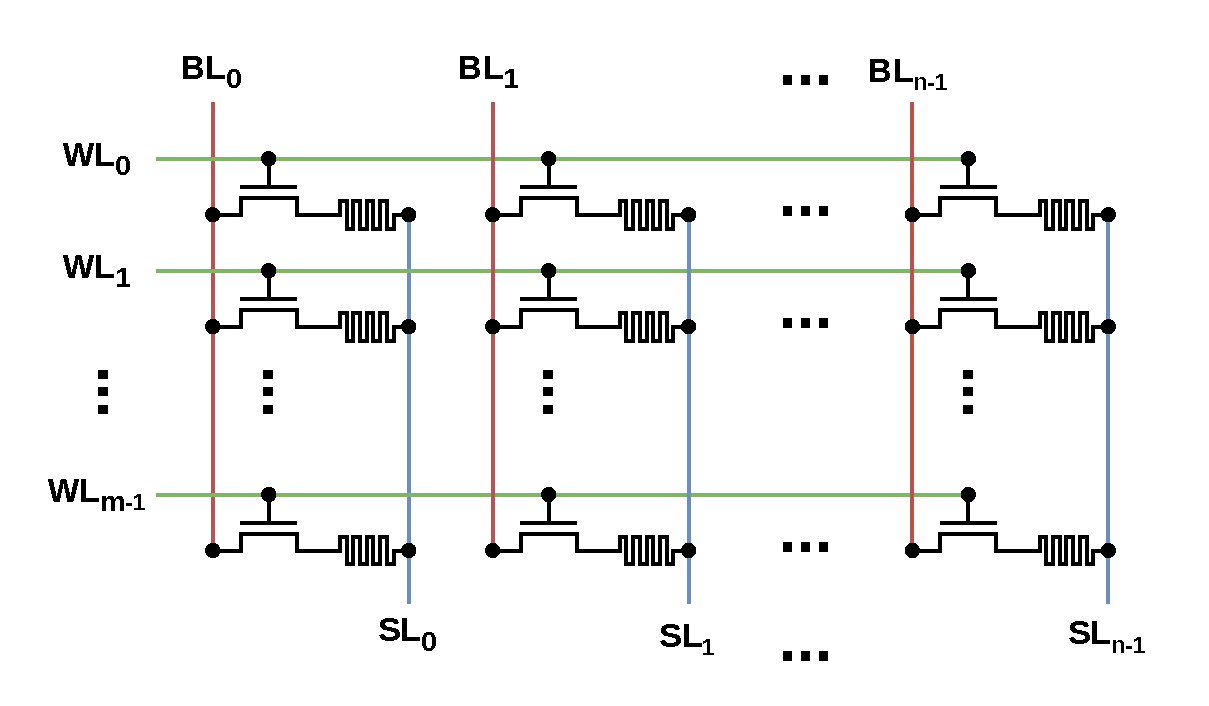
\includegraphics[width= 0.9\linewidth]{img/ReRAM-1T1R-Xbar.pdf}
	\caption{A conventional 1T-1R ReRAM crossbar array. \label{fig:xbar}}
\end{figure}



Bipolar switching imposes strict constraints on how SET and RESET
operations can be applied within a crossbar array. SET and RESET
operations require opposite voltage polarities across the switching
layer, and the shared WL and BL rails of a crossbar architecture
typically cannot apply both polarities simultaneously to different cells
in the same word~\cite{xu2015overcoming, mao2016optimizing}. As a
result, write controllers must serialize SET and RESET phases: all cells
requiring a SET transition within a word are programmed in one phase,
and all cells requiring a RESET transition are programmed in a separate
phase. A write operation that requires both polarities within a single
word therefore incurs the latency of two sequential programming phases,
while a write requiring only one polarity incurs a single phase.

The impact of polarity serialization on write latency can be
characterized by the directional Hamming distance (DHD) of a codeword
transition. For a write from codeword $c_0$ to codeword $c_1$, the DHD
is a tuple $(w_{0\to1}, w_{1\to0})$ counting the number of positive
(SET) and negative (RESET) bit transitions respectively. A write with
$w_{0\to1} = 0$ or $w_{1\to0} = 0$ requires only a single programming
phase and produces a unipolar write latency. A write with both
$w_{0\to1} > 0$ and $w_{1\to0} > 0$ requires both phases and produces a
bipolar write latency, which is the maximum observed $t_w$ for a given
word. A redundant write with $w_{0\to1} = w_{1\to0} = 0$ requires no
transitions and produces the minimum observed $t_w$. The DHD of the
codeword transition, not the user-visible dataword transition,
determines the write latency category, because ECC parity bit activity
contributes transitions that are not visible in the data.

When an ECC is present, parity bits are computed over the data word and
appended to form a codeword before programming. The parity bit
transitions required for a given data write depend on the parity
submatrix of the code and the specific data transition being performed.
These parity-driven transitions modify the DHD of the effective codeword
write, potentially promoting a unipolar data transition to a bipolar
codeword transition or changing the number of transitions in each
polarity. Because the ECC structure is not disclosed by vendors, the
contribution of parity activity to write latency is not predictable from
the data word alone. This is the fundamental obstacle to accurate timing
modeling and rigorous entropy characterization in commercial ReRAM, and
the core motivation for ECC recovery.